\def\mytitle{\textbf{ARM ASSIGNMENT}}
\documentclass[10pt,a4paper]{article}
\usepackage[a4paper,outer=1.5cm,inner=1.5cm,top=2cm,bottom=1.5cm]{geometry}
\usepackage{float}
\usepackage{amsfonts}
\usepackage{titlesec}
\usepackage[utf8]{inputenc}
\usepackage{textgreek}
\usepackage{tabularx}
\usepackage{graphicx}
\title{\mytitle}
\author{Pavan Srinivas Marri\\marripavan65@gmail.com\\FWC22138 IITH - Future Wireless Communications}
\date{}
\begin{document}
\maketitle
\tableofcontents
\graphicspath{{./Documents}{./figs}}
\section{Problem}
(GATE2020-QP-EE)\\
Q.54 An 8085 microprocessor acesses two memory locations $(2001H)$ and $(2002H)$, that contains $8$-bit numbers $98H$ and $B1H$ , respectively. the following program is executed:\\
     LXI H,$2001H$\\
     MVI A,$21H$\\
     INX H \\
     ADD M \\
     INX H \\
     MOV M,A \\
     HLT \\
     At the end of this program ,the memory location $2003H$ contains the number in decimal(base $10$ ) form\\
     \section{Components}
     \begin{table}[H]
	     \centering
	     \begin{tabularx}{1\textwidth}
			{
				| >{\centering\arraybackslash}X
				| >{\centering\arraybackslash}X
				| >{\centering\arraybackslash}X |}
			\hline
			{\bf Components} & {\bf Value} & {\bf Quantity} \\
			\hline
			Breadboard & - & 1\\
			\hline
			Jumper Wires & - & 20 \\
			\hline
			LCD & 16x2 & 1\\
			\hline
			Vaman & - & 1\\
			\hline
		\end{tabularx}
			\caption{Components}
			\label{table=Components}
     \end{table}
     \section{Implementation}
     \subsection{Solution}
     LXI H, 2001H; H = 20 H, L = 01 H \\
     MVI A, 21H; A = 21 H \\
     INX H; HL + 1 $ \rightarrow $ H = 20 H $ \rightarrow $ HL = 2002 H \\
     ADD M; [A] + Reference data of HL pair = 21 H + B1 H = D2H $ \rightarrow $ [A] \\
     INX H; [HL] + 1 $ \rightarrow $ 2002 H + 1 H $ \rightarrow $ 2003H  \\
     MOV M, A; [A] to Memory, reference of HL pair, 2003 H [D2] $ \beta $ [D2] = A \\
     HLT; Stop
     Therefore, content in the 2003 H is D2H \\
     Converting in decimal \\
     D x $ 16^1 $ + 2 x $ 16^0 \rightarrow $ 13 x 16 + 2 = $ (210)_{10} $
     \section{Hardware}
     \subsection{Vaman to LCD connections}
     \begin{table}[H]
	     \begin{tabularx}{1\textwidth} {
	| >{\centering\arraybackslash}X
	| >{\centering\arraybackslash}X
	| >{\centering\arraybackslash}X
	| >{\centering\arraybackslash}X |}
		\hline
		Pygmy & LCD pins & LCD pin label & LCD pin Description \\
		     \hline
		     GND & 1& GND & \\
 		\hline
 		5V & 2 & Vcc &\\
 		\hline
 		GND & 3 & Vee & Contrast\\
		 \hline
 		10 & 4 & RS & Register Select\\
 		\hline
		 GND & 5 & R/W & read/write\\
		 \hline
		 9 & 6 & EN &Enable\\
		 \hline
		 14 & 11 & DB4 & Serial connection\\
		 \hline
		 13 & 12 & DB5 & Serial connection\\
		 \hline
		 12 & 13 & DB6 & Serial connection\\
		 \hline
		 11 & 14 & DB7 & Serial connection\\
		 \hline
		 5V & 15 & LED+ & Backlight\\
		 \hline
		 GND & 16 & LED- & Backlight\\
		 \hline
	     \end{tabularx}
	     \caption{Vaman to LCD}
	     \label{table:connections}
     \end{table}
     \begin{figure}[H]
	     \centering
	     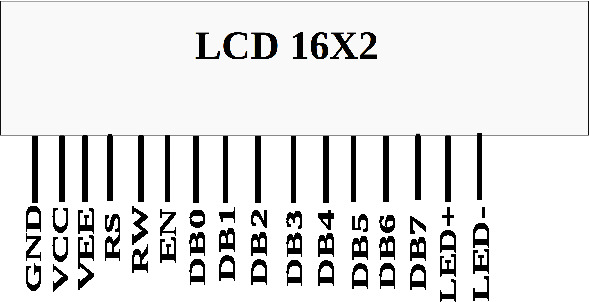
\includegraphics[scale=0.4]{figs/lcd.jpg}
	     \caption{LCD pins}
	     \label{fig:LCD}
     \end{figure}
     \subsection{Procedure}
     \begin{enumerate}
	     \item Make the coneection to the vaman and LCD as in the table above.
	     \item Refer fig:1 for the reference of LCD pins.
	     \item Connect the Vaman to the PC via USB and dump your code into vaman.
     \end{enumerate}
     \subsection{LCD output}
     \begin{figure}[H]
	     \centering
	     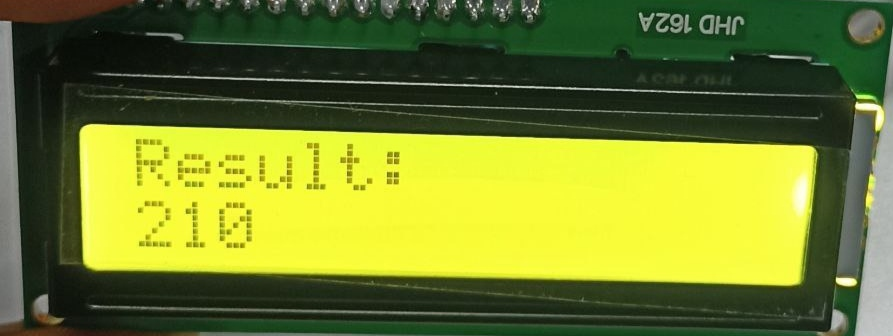
\includegraphics[scale=0.5]{figs/lcd1.jpg}
	     \caption{Output}
	     \label{fig:output}
     \end{figure}
     \section{Software}
	Execute the code which is available in the below path and upload it to the Vaman. \\
	\framebox{https://github.com/Pavan2k01/Digital-Design/blob/main/ARM/main.c}
     \section{Conclusion}
	Hence, We have executed the above code using Vaman in ARM environment.
\end{document}
